\chapter{Medien im Unterricht}\label{Medien}

\section{Grundlagen}
\subsection{Begriff}
Engerer (praktischer) Begriff (Fr\"{o}hlich, 1974): Medien sind
\begin{itemize}
\item
technische Unterrichtshilfen, die der Lehrer einsetzt oder
\item
Lernmittel f\"{u}r die Hand der Sch\"{u}ler.
\end{itemize}

Im weiteren Sinne k\"{o}nnte man als Medium all das bezeichnen, was der
Informations\"{u}bertragung und -bewahrung dient:
Die Luft als Tr\"{a}germedium
des Schalls und des Lichts, das gesprochene Wort \dots.

\subsection{Ziele beim Einsatz von Medien}
\begin{itemize}
\item
Informationsvermittlung und -bewahrung
\item
Veranschaulichung: ,,Ein Bild sagt mehr als tausend Worte'',
Modellger\"{a}te, Modellversuche
\item
Entlastung des Lehrers von Routine\-t\"{a}tigkeiten zugunsten einer
p\"{a}dagogischen T\"{a}tigkeit
\item
Lebensn\"{a}he
\item
Differenzierung im Klassenunterricht, Steuerung
im Gruppenunterricht
\item
Vielf\"{a}ltige Variation des Unterrichtsgeschehens
\end{itemize}

\subsection{\"{U}berblick \"{u}ber typische Medien}
\begin{itemize}
\item Analoge Tafeln aller Art:
	\begin{itemize}
	\item Wandtafel (Kreidetafel)
	\item Lehrtafeln (Landkarten, Tabellen (PSE, Isotopen\-karte))
	\item Pinnwand
	\item Magnet\-haft\-ta\-fel
	\end{itemize}

\item Derzeit übliche AV-Ausstattung in Schulen
	\begin{itemize}
		\item ortsfester PC oder Laptop
		\item Beamer oder großer Bildschirm
		\item Dokumentenkamera
		\item Soundanlage
		\item Bring your own Device (BYOD): Lehrkraft bringt eigenes Gerät (i. d. R. Tablet) mit ins Klassenzimmer und kann dieses über Kabel oder drahtlos auf den Beamer spiegeln
		\item immer häufiger: Smartboards
	\end{itemize}

\item Weitere Medien
	\begin{itemize}
		\item Tageslichtprojektor
		\item CD-Spieler
		\item Bluetooth-Box
	\end{itemize}
\item Digitale Lernplattformen
	\begin{itemize}
		\item ByCS/mebis
		\item Teams
	\end{itemize}

%\item
%Projektoren aller Art:
%\begin{itemize}
%\item
%Tageslichtprojektor (TLP oder OHP),
%\item
%Video-Anlage, Diaprojektor, Filmprojektor, Episkop sind angesichts der Pr\"{a}senz von Computertechnologie praktisch verdr\"{a}ngt. \end{itemize}
%\item
%Audio-Ger\"{a}te aller Art:
%\begin{itemize}
%\item
%CD-Player (Akustik, Schwebungen).
%\item
%Tonbandger\"{a}t, Kassettenrekorder, Plattenspieler, Radioger\"{a}t (Schulfunk) finden sich heute kaum noch in der Schulpraxis.
%\end{itemize}
\end{itemize}

\section{Analoges Medium: die Wandtafel}
\begin{itemize}
\item Mittelpunkt: Die Tafel ist auch heute oft noch das Medium, das im
Mittelpunkt des Unterrichts steht,
symbolisch entspricht dies der Anordnung der Tafel in
der Mitte der Stirnseite des Klassenzimmers.

\item Dynamik: Das Tafelbild wird w\"{a}hrend einer Stunde entwickelt
und spiegelt daher die Dynamik eines Unterrichts\-verlaufs wider.

\item Planung: Meist wird es mehr oder weniger genau --- eventuell
ma{\ss}st\"{a}blich --- geplant.
Es enth\"{a}lt dann in m\"{o}glichst pr\"{a}gnanten, klaren Formulierungen einen
auch f\"{u}r den Sch\"{u}ler-Hefteintrag geeigneten Lehrtext
und zugeh\"{o}rige Skizzen, Zeichnungen oder Diagramme.

\item Spontaneit\"{a}t: Es kann aber auch spontan entwickelt werden
(Nebenrechnungen, Skizzen, Kurzerkl\"{a}rungen, Messwerte,\dots).
\end{itemize}

\bip
Hinweise zur Arbeits\-technik  an der Wandtafel:
\begin{itemize}
\item
Die Tafel sollte mit einem sauberen Lappen gewischt und dann
trocken sein.
\item
Achte auf gute Sichtverh\"{a}ltnisse: Beleuchtung der Tafel
m\"{o}glichst von vorne oben, Unterbindung von Reflexionslicht.
\item
Achte bei der Planung auf Eigenschaften der Tafel:
Gr\"{o}{\ss}e der Teiltafeln, Klappm\"{o}glichkeiten, Skalierung der K\"{a}stchen,
Befestigungsm\"{o}glichkeiten (Haken, Stative, Magnetclips)
Korrektur nach Trockenwischen, Annahme von Farbkreide.
\item
Soll die Tafel (grunds\"{a}tzlich) bez\"{u}glich verschiedener
Funktionen unterteilt werden: Konzepttafel, Nebenrechnungen,
Hefteintrag,\dots

\item
Spreche nicht zur Tafel! Stehe seitlich zur Schreibhand!
Quietschende Kreide sollte durchgebrochen werden.
\item
Achte auf den Zeitbedarf!
Das Tempo beim Tafelschreiben ist von selbst eher sch\"{u}lergem\"{a}{\ss}.
\item
Zeichnungen:
\begin{itemize}
\item
Beim Zeichnen von Kurven ist die Richtung von oben nach
unten g\"{u}nstiger!
\item
Die Hand sollte ---  unverkrampft --- in etwa senkrecht
zur momentanen Strichrichtung ausgerichtet sein.
\item
Arbeite m\"{o}glichst mit Hilfspunkten und/oder Symmetrien.
\item
Dr\"{u}cke Zeichenwerkzeuge immer in der N\"{a}he des aktuellen
Zeichnens an!
\item
Bei perspektivischen Darstellungen ist \"{U}bung (evtl.\ vorher
auf dem Papier) von Vorteil.
Entwickle die Darstellung bez\"{u}glich der Richtung senkrecht zur
Tafel ,,in die Tafel hinein'' (wegen der Verdeckungsrelationen)!
\mip
\"{U}bung: Zeichne einen Hufeisenmagneten, eine Spule
mit Andeutung der Windungsrichtungen, einen Quader (W\"{u}rfel),
eine Kugel.
\end{itemize}
\item
Falsches (Beispiele f\"{u}r typische Fehler) sollte als solches
kenntlich sein.
\end{itemize}

Spezielle Hinweise f\"{u}r Mathematik und Physik:
\begin{itemize}
\item
Der Kreidezirkel sollte in der N\"{a}he der Saugn\"{a}pfe
festgehalten werden.
Der Kreismittelpunkt muss vor dem Kreiszeichnen markiert werden
(Es gibt keinen Einstichpunkt).
\item
Beim Zeichnen von geometrischen Figuren oder Graphen
(Messwerte, Funktionsgraphen) arbeite man mit Hilfspunkten oder
Symmetrien! Werden Punkte eines Graphen mit $+$ statt $\times$ markiert,
so sind sie nach der Fertigstellung des Graphen leichter
erkennbar.
\item
Bei einem drei-dimensionalen  Koordinatensystem sollte die
zur Tafelebene senkrechte Achse nach vorne gezeichnet sein.
Dann wird sie nicht von Objekten im Quadranten der anderen beiden
Achsen verdeckt.
\item
Verwendung von ,,Icons'':
Auge, Mikroskop, Motor,\dots

\item
Verwendung von Symbolen: Schaltbilder von el.\ Schaltungen,
Befestigungen.
\end{itemize}

\section{Digitale Medien}
\subsection{Grundlagen: das SAMR-Modell}
\begin{figure}
	\centering
	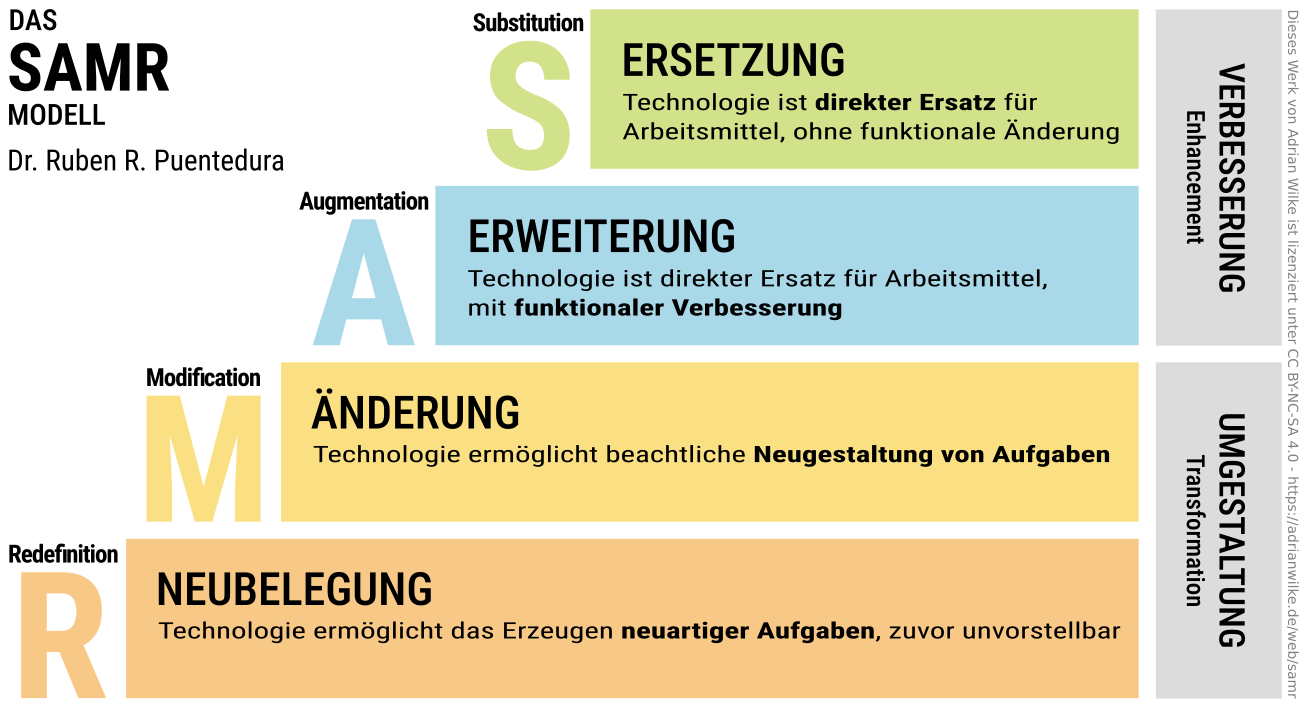
\includegraphics[width=.9\textwidth]{SAMR-Puentedura-deutsch.png}
	\caption{Das SAMR-Modell nach Puentedura}\label{fig:samr}
\end{figure}

Digitale Medien\footnote{Wir können hier nur einen knappen Einblick in spezifische Aspekte geben. Darüber hinaus verweisen wir auf die Veranstaltungen \emph{Lehren und Lernen mit und über digitale Medien} bei Dr. Seyferth-Zapf sowie \emph{Erstellung videobasierter LearningBits} aus unserem Kanon.} ergänzen den Einsatz analoger Medien sinnvoll und verdrängen diese teilweise bereits. Einen theoretischen Rahmen bildet das in \cref{fig:samr} illustrierte SAMR-Modell nach Dr. Ruben R. Puentedura, das die Integration von Technologie im Unterricht in vier Stufen beschreibt:
\begin{enumerate}
	\bitem{Substitution (Ersetzung)} Technologie ersetzt herkömmliche Werkzeuge, ohne grundlegende Änderungen am Unterrichtsprozess.
	\bitem{Augmentation (Erweiterung)} Technologie ersetzt herkömmliche Werkzeuge und bietet funktionale Verbesserungen.
	\bitem{Modification (Modifikation)} Der Einsatz von Technologie führt zu einer Umgestaltung der Lernaktivitäten.
	\bitem{Redefinition (Neudefinition)} Technologie ermöglicht völlig neue Lernformen, die ohne sie nicht möglich wären.
\end{enumerate}

\begin{beisp2}
	\begin{enumerate}
		\item Ein gedrucktes Arbeitsblatt wird durch ein digitales Dokument ersetzt.
		\item Das digitale Dokument enthält interaktive Elemente wie Links oder Kommentare.
		\item Lernende bearbeiten Projekte kollaborativ in Echtzeit über Online-Plattformen.
		\item Lernende erstellen Videos oder interaktive Präsentationen, um komplexe Konzepte zu vermitteln und weltweit zu teilen.
	\end{enumerate}
\end{beisp2}

Das Modell dient als Leitfaden, um den Einsatz von Technologie im Unterricht zu reflektieren und gezielt zu verbessern.

\subsection{Das Tablet als Tafel}
Tablets mit digitalen Stiften werden heute häufig für Tafelanschriebe verwendet. Dabei verwendet man eine Notizen-App wie Goodnotes oder das an vielen Schulen eingesetzte Microsoft OneNote. Der Tablet-Bildschirm wird auf den Beamer oder großen Bildschirm gespiegelt.

\mip
Grundlegend gelten dieselben Argumente wie für die Entwicklung eines Hefteintrags an der Kreidetafel, die Verwendung eines Tablets hat jedoch folgende \textbf{Vorteile} (=Augmentation):
\begin{itemize}
	\item Der Lehrer schaut zur Klasse.
	\item Das Geschriebene ist konserviert und kann 	ausgewertet, archiviert oder wiederverwendet (Wiederholung) werden. Entsprechende Apps erlauben den Export als PDF, sodass der Hefteintrag der Klasse digital zur Verfügung gestellt werden kann.
	\item Beinahe unendliche Kapazit\"{a}t. Die \say{Tafel} muss nicht gewischt werden.
	\item Beliebige Vielfalt bei den Vorlagen: Kariertes Papier, Koordinatensystem, Leertabelle, L\"{u}ckentext.
	\item Bilder können eingefügt und direkt beschriftet werden.
	\item
	Die Farbgebung ist einfacher.
	Die Zuordnung hell/dunkel bzgl.\ des Sch\"{u}lerhefteintrags stimmt
	(dunkel auf der Folie $\Rightarrow$ dunkel im Heft).
	\item Direkter Zugriff auf digitale Ressourcen wie Bilder, Animationen, Simulationen, Filme, \dots ohne Umschalten.
	\item Arbeisblätter können gemeinsam ausgefüllt werden.
\end{itemize}

Es gibt jedoch auch \textbf{Nachteile:}
\begin{itemize}
	\item Reizüberflutung der Schüler durch Übertechnisierung
	\item Tun des Lehrers nicht so gut erkennbar, nur Textentstehung, erschwert Nachahmung
	\bitem{Warnung} Man neigt im Digitalen zur Vorwegnahme, z. B. durch vorgefertigte Präsentationen. Dies kann den Konstruktionsprozess der Schüler behindern.
\end{itemize}

\subsection{Das Smartboard}
Ein Smartboard ist eine digitale Tafel, die Eigenschaften von Kreidetafel und Tablet auf sich vereint: Mit dem Finger oder mit digitalen Stiften kann auf ihrer Oberfläche geschrieben werden. Zudem können weitere Inhalte (z. B. Graphiken) eingebunden werden.

\begin{itemize}
	\item Aufgrund der Ähnlichkeit zur Kreidetafel gelten dieselben Warnhinweise wie für diese analog.
	\item Der Umgang mit Smartboard-Systemen ist häufig auch für Digital Natives nicht intuitiv und muss geübt werden. Ein \say{Kampf mit der Technik} ist eine der wesentlichsten Unterrichtsstörungen.
	\item In unserem Klassenzimmer \say{Luki} ist ein Smartboard verbaut, an dem Ihr gerne üben könnt.
\end{itemize} 

\subsection{Die Dokumentenkamera}
Eine Dokumentenkamera ist ein digitales Präsentationsgerät, das gedruckte oder physische Materialien in Echtzeit auf eine Projektionsfläche oder einen Bildschirm überträgt. Sie ermöglicht es Lehrkräften, Bücher, Arbeitsblätter oder Objekte visuell zu präsentieren und zu vergrößern, wodurch detaillierte Erklärungen vor einer größeren Gruppe möglich werden. Zudem kann sie oft mit anderen Geräten wie Computern oder interaktiven Whiteboards verbunden werden, um das gezeigte Material digital zu speichern oder weiterzubearbeiten.

\mip
Ihr Einsatz eignet sich besonders dann, wenn \dots
\begin{itemize}
	\item analoge Schülerarbeiten der Klasse gezeigt werden sollen, z. B. bei der Besprechung der Hausaufgabe oder der Bearbeitung eines Arbeitsblattes.
	\item die feinmechanische Vorgehensweise relevant ist, z. B. beim Eintragen von Messwerten in Diagramme.
	\item der Umgang mit Instrumenten gezeigt wird, z. B. die Einstellung des Messbereichs und das korrekte Ablesen der Messdaten bei Analogmultimetern.
\end{itemize}

\subsection{Der Tageslichtprojektor}
Heutzutage handelt es sich eher um ein Relikt, eine Vorstufe zu den vorgenannten Medien. Dennoch ist er nützlich zur Projektion mancher Experimente:

\begin{itemize}
	\item
	Mit dem TLP steht grunds\"{a}tzlich eine intensive
	Lichtquelle zur Verf\"{u}gung.
	\item
	Der TLP kann als Projektionslampe zum Schattenwerfen dienen:
	Kreisbewegung wird als harmonische Schwingung gesehen.
	Schatten einer Kerzenflamme.
	\item
	Anzeigeger\"{a}te mit transparenter Skala (Messinstrumente, Kompass)
	\item
	Licht-Schatten-Ph\"{a}nomene
	\item
	Mechanisch dynamische Vorg\"{a}nge: Sto{\ss}en, Ablenken,
	Stahlnagel-Elektromagnet, Oersted-Versuch.
	\item
	Farbmischung (Subtraktiv bei farbigen Folien)
\end{itemize}

\subsection{Aspekte des Einsatzes von Computern im Physikunterricht}

\begin{itemize}
	\bitem{Als klassisches AV-Medium} Bilder, Filme, Animationen, Simulationen, PowerPoint-Präsentationen, \dots
	\bitem{Schulung von Medienkompetenz} Als schulart- und fächerübergreifendes Bildungs- und Erziehungsziel ist Medienbildung und digitale Bildung auch im Physikunterricht relevant.
	\begin{itemize}
		\item Bedienung physikspezifischer Programme: Experimentierumgebungen, Datenerhebung und -auswertung (PhET, Excel, GeoGebra, \dots)
		\item Bewertung von Internetquellen hinsichtlich ihrer Glaubwürdigkeit
		\item Recherchemöglichkeiten im Internet
		\item Gestaltung ansprechender Präsentationen, z. B. mit PowerPoint
	\end{itemize}
	\bitem{Schulung von Programmierfähigkeiten} In der Zusammenarbeit mit Mathematik und Informatik ist algorithmisches Denken auch in der Physik wichtig. Programmierfähigkeiten lassen sich bspw. bei der Umsetzung der Methode der kleinen Schritte schulen.
	\bitem{Computer als Unterrichtsgegenstand} Physikalische Grundlagen heutiger und zukünftiger Computertechnologie
	\bitem{Digitale Messwerterfassung}
	\begin{itemize}
		\item Eine Vielzahl von digitalen Sensoren (Bewegung, Lichtschranken, Kraft, Druck, Schall, Stromstärke, Spannung, Temperatur, Magnetfeld, \dots) lassen sich über USB oder drahtlos mit dem PC verbinden und die Daten auslesen.
		\item Verbreitete Systeme: \textbf{CASSY, Phywe, Vernier}
		\item Zugriff auf Primär- und Sekundärdaten (z. B. Ort und Geschwindigkeit durch Integration über Daten des Beschleunigungssensors) mittels geeigneter Software
		\item Direkte Darstellung der erhobenen Daten in Tabellen oder Diagrammen
		\item Speicherung der Messergebnisse
		\item Vorteile:
			\begin{itemize}
				\item Schnelle, bequeme Bedienbarkeit $\to$ Zeitersparnis.
				\item Vielseitigkeit: Vergleiche oben.
				\item \"{U}bersichtliche Aufbewahrung $\to$ Platzersparnis.
				\item Standardisierung,
				\item Blackbox-Prinzip: Der wesentliche Gehalt eines Experiments kann besser herausgearbeitet werden.
				\item Verfügbarkeit und Portabilität der Daten: Ergebnisse eines Lehrerexperiments können Schülern zur weiteren Analyse zur Verfügung gestellt werden.
			\end{itemize}
		\item Nachteile:
			\begin{itemize}
				\item Die Unmittelbarkeit der messenden Erfassung von physikalischen Ph\"{a}nomenen geht verloren.
				\item Handwerkliche Fertigkeiten werden in den Hintergrund gedr\"{a}ngt.
				\item Zunehmende Abh\"{a}ngigkeit von ausgefeilten Technologien.
				\item Kosten f\"{u}r Neuanschaffungen. Eigentlich sind Messwerterfassungssysteme vergleichsweise billig.
				\item Blackbox-Prinzip: Messprinzip kann verschleiert werden.
			\end{itemize}
	\end{itemize}
\end{itemize}

\section{K\"{u}nstliche Intelligenz \`{a} la ChatGPT --- speziell im Physikunterricht}

ChatGPT und verwandte Angebote zur Nutzung k\"{u}nstlicher Intelligenz sind erst k\"{u}rzlich allgemein zug\"{a}glich geworden, erfreuen sich aber bereits allergr\"{o}{\ss}ter Beliebtheit insbesondere bei Sch\"{u}lerinnen und Sch\"{u}lern, sowie Studenten. Die Entwicklung der k\"{u}nstlichen Intelligenz steht noch am Anfang, sodass damit zu rechnen ist, dass sich die zur Verf\"{u}gung stehenden M\"{o}glichkeiten und die Qualit\"{a}t der Ergebnisse stetig weiterentwickeln werden. Auf eine Darstellung, was ChatGPT ist und wie man es benutzt, wird hier verzichtet. Vielmehr sollen hier Ideen skizziert werden, auf welche Weise ChatGPT gewinnbringend im Physikunterricht eingesetzt werden kann.

\begin{enumerate}
\item \textbf{Generieren von Inhalten:} ChatGPT kann mit gro{\ss}er Leichtigkeit Texte und eine Vielzahl von Grafiken erzeugen. 
	\begin{beisp} 
	\say{\emph{Erstelle mir eine kurze Zusammenfassung zum Film \say{The Fast and the Furious}, die ich in einer dreimin\"{u}tigen Pr\"{a}sentation in der Schule verwenden kann, im Sprachstil von Letty Ortiz!}}
	\end{beisp}

\item \textbf{Study-buddy:} Sch\"{u}ler k\"{o}nnen  mit ChatGPT interaktiv und im eigenen Tempo \"{U}bungsfragen durchgehen und Rechenaufgaben l\"{o}sen. Physikalische Konzepte k\"{o}nnen durch ChatGPT verst\"{a}ndlich erkl\"{a}rt werden und im Dialog mit ChatGPT erlernt werden. Im Gegensatz zu Google ist KI in der Lage, einen Dialog mit dem Bedienenden zu f\"{u}hren, auf Fragen zu antworten, auf Nachfrage zu pr\"{a}zisieren, Beispiele zu liefern, Gegenbeispiele zu liefern usw.. ChatGPT kann somit als Gespr\"{a}chspartner in simulierten Diskussionen \"{u}ber physikalische Themen dienen. 
	\begin{beisp}
	\glqq\emph{Nenne mir ein Experiment, mit dem nachgewiesen wird, dass die Ladung des Elektrons wirklich negativ ist!}\grqq,  analysiere die generierte Antwort kritisch, und stelle Folgefragen, beispielsweise \glqq\emph{Wird durch dieses Experiment wirklich das Vorzeichen der Ladung ermittelt?}\grqq.  
	\end{beisp}

\item \textbf{Ideengeber bei Hausaufgaben und Projekten:} Sch\"{u}ler k\"{o}nnen ChatGPT nutzen, um Unterst\"{u}tzung bei Hausaufgaben, Projektideen oder der Recherche nach Informationen zu physikalischen Themen zu erhalten. 
	\begin{beisp} 
	\glqq\emph{Nenne mir drei Experimente zum Nachweis des Strahlencharakters von Licht f\"{u} den Physikunterricht der 8. Klasse!}\grqq
	\end{beisp}

\item \textbf{Begutachtung von schriftlichen Arbeiten und Vorbereitung auf Pr\"{u}fungen:} Sch"{u}ler k\"{o}nnen ChatGPT nutzen, um sich auf Pr\"{u}fungen vorzubereiten, indem sie Fragen stellen, Erkl\"{a}rungen wiederholen und gezielte R\"{u}ckmeldungen zu ihren Antworten erhalten. ChatGPT kann als virtueller Gutachter verwendet werden, um eigene Textentw\"{u}rfe zu begutachten. 

	\begin{beisp} 
	Ziehen Sie eine pdf-Datei mit einer selbsterstellten Ausarbeitung oder auch eine Grafik in den Eingabeprompt und bitten Sie um eine Zusammenfassung oder eine Analyse bzw. Bewertung!
	\end{beisp}
	
	
\item \textbf{Unterst\"{u}tzung f\"{u}r Lehrkr\"{a}fte:} Lehrer k\"{o}nnen ChatGPT als Hilfsmittel bei der Unterrichtsvorbereitung einsetzen, z.B. zum Erstellen von \"{U}bungsaufgaben, zur schnellen Recherche oder als Inspirationsquelle f\"{o}r neue Unterrichtsideen. 
	\begin{beisp2}
	\begin{itemize}
	\item {\glqq}\emph{Gib die erforderlichen Lernvoraussetzungen, Lernziele und eingesetzte Medien in einer Unterrichtsstunde zum Fadenstrahlrohr an.}{\grqq} 
	\item {\glqq}\emph{Gestalte eine sch\"{u}lerzentrierte Unterrichtseinheit zum Thema elektrische Influenz in der Mittelstufe. W\"{a}hle ein Artikulationsschema des entdeckenden Unterrichts. Gehe explizit auf Vorwissen und Lernziele ein und verdeutliche, wie durch die Ma{\ss}nahmen dieser Unterrichtseinheit die gesetzten Lernziele erreicht werden k\"{o}nnen.}{\grqq} 
	\end{itemize}
	\end{beisp2}
\end{enumerate}
\bip

ChatGPT erm\"{o}glicht  nicht nur effizientes und kreatives Arbeiten, ebenso kann ChatGPT  den Physikunterricht bereichern, indem es personalisierte Lernm\"{o}glichkeiten bietet  und den Zugang zu komplexen Inhalten vereinfacht. Durch die Verwendung von ChatGPT wird das selbstgesteuerte Lernen stark gef\"{o}rdert und eine Bef\"{a}higung zum zum kritischen und ausgiebigen Dialog angestrebt.
\mip
Es ist jedoch darauf zu achten, dass der Einsatz von ChatGPT bewusst gesteuert wird, um sicherzustellen, dass es als Erg\"{a}nzung und nicht als Ersatz f\"{u}r den direkten Unterricht und die zwischenmenschliche Interaktion dient. Beim Generieren von Inhalten wird die Eigenleistung der Lernenden im kreativen Recherche- und Schreibprozess umgangen. Lehrkr\"{a}fte m\"{u}ssen sich mit den M\"{o}glichkeiten durch ChatGPT vertraut machen und klare Regeln zu dessen Anwendung aufstellen.
\mip
Letztlich muss gewarnt werden, dass ChatGPT gelegentlich zum {\glqq}Halluzinieren{\grqq} neigt, d.h. dass es frei erfundene Antworten erzeugt. Output von ChatGPT sollte daher niemals  ungepr\"{u}ft \"{u}bernommen werden. 

\section{Schriftliche Medien --- f\"{u}r die Hand der Sch\"{u}ler}
\subsection{Das Schulbuch}

\subsection{Arbeitsbl\"{a}tter und -hefte}
\begin{itemize}
\item
Selbstgestaltet --- vorgefertigt.
\item
Inhalte k\"{o}nnen korrekt und auf den Punkt gebracht
dargestellt werden.
\item
Gestaltung individuell: Tabellen, Diagramme, Bilder, Skizzen.
\item
M\"{o}gliche Sch\"{u}leraktivit\"{a}ten (Begleitet auf der Folie):
\begin{itemize}
\item
Erg\"{a}nzung: L\"{u}ckentexte, Tabellen, Zeichnungen.
\item
Farbige Gestaltung: Texte markieren, Skizzen f\"{a}rben,
           Zeichnungs\-tei\-le kennzeichnen.
\item
Beschriften von Zeichnungen, Diagrammen.
\item
Grafische Gestaltung: Unterstreichen, Einrahmen, Schraffieren.
\end{itemize}

\item
\"{O}konomie: Zeitersparnis im Unterricht, in der Vorbereitung.
\item
Arbeitsblatt-Verwaltung durch den Lehrer:
Heute mit PC m\"{o}glich und vielf\"{a}ltig.

\item
Probleme:
\begin{itemize}
\item
,,Zettelwirtschaft'' bei Sch\"{u}lern (G\"{u}nstig: Nummerierung, Datumsangabe (Kieserblock).
\item
Eine beim Lehrer hervorgerufene ,,Stoffabarbeitungs-Philosophie''
korrespondiert mit einem Minimal-Aufwand an Vorbereitung.
Im Unterricht ruft dies einen Eindruck von Eint\"{o}nigkeit hervor.
(Es gibt Verlage, die genau diese Art von Lehrermentalit\"{a}t bedienen:
,,Da brauchen Sie nur noch in der Fr\"{u}h schnell kopieren''.)
\end{itemize}
\end{itemize}

\subsection{Das Sch\"{u}lerheft}

Praktische Hinweise f\"{u}r Zeichnungen:
\begin{itemize}
\item
Beim Zeichnen von Kurven/Graphen setze den Handballen in der
N\"{a}he auf und ziehe den Strich in Schreibrichtung!
Eventuell sollte vorher das Heft gedreht werden.

\item
Zeichnungen sollten nach M\"{o}glichkeit mit
Bleistift angefertigt werden,
da dann das Radieren m\"{o}glich ist.
(Auch wegen Verdeckungen muss manchmal radiert werden.)
\end{itemize}

